\documentclass[sigconf, proceedings, 9pt]{acmart}
\settopmatter{printacmref=false} % Removes citation information below abstract
\renewcommand\footnotetextcopyrightpermission[1]{} % removes footnote with 
%conference information in first column
\usepackage{bigstrut}
\usepackage{amsmath}
\usepackage{balance}
\usepackage{dsfont}
\usepackage{booktabs}
\usepackage{multirow}
\usepackage[english]{babel}
\usepackage{blindtext}
\usepackage{enumitem}
\setlist{leftmargin=*}
\definecolor{Code}{rgb}{.12,.79,.17}
\definecolor{steel}{rgb}{0.4, 0.4,0.7}
\definecolor{Green}{rgb}{.12,.79,.17}
\usepackage{tikz}
\usepackage{calc}
\linespread{1.1}
\def\checkmark{\tikz\fill[scale=0.3](0,.35) -- (.25,0) -- (1,.7) -- (.25,.15) 
-- cycle;} 
\def\scalecheck{\resizebox{\widthof{\checkmark}*\ratio{\widthof{x}}{\widthof{\normalsize
 x}}}{!}{\checkmark}}
%\usepackage[table,dvipsnames]{xcolor}
\usepackage{colortbl}
\newcommand{\gray}{\rowcolor[gray]{.95}}
\setlength{\arrayrulewidth}{0.5pt}
\pagenumbering{arabic}
\renewcommand{\i}{\item}
\newcommand{\tion}[1]{\S~\ref{sect:#1}}
\newcommand{\fig}[1]{Fig.~\ref{sect:#1}}
\setlength{\abovedisplayskip}{4pt}
\setlength{\belowdisplayskip}{4pt}
\def\bibfont{\small}

\begin{document}
\title{On Recommending Actionable Changes\\For Software Projects}
\author{Rahul Krishna}
\affiliation{NC State University}
\email{i.m.ralk@gmail.com}
%\acmDOI{}
%\acmISBN{}
\acmPrice{}
\acmConference[Fss'17]{}{Foundations of Software Science}{Fall 2017.}{}

\maketitle

\section{Criteria}
In order to assess this project the following criteria will be explored. The 
proposed software analysis tool to be used in this project is XTREE. Listed 
below are some of the criteria that are used to assess a software analytics 
tool. Of these, some of the criteria are already satisfied by XTREE. The focus 
of this project will be to attempt to address some of relevant aspects from 
below that are not currently supported.

\begin{enumerate}[noitemsep,topsep=0pt]
	\item \textit{\textbf{Model Readability:}}
	The proposed software analysis tool to be used in this project (XTREE) address 
	this problem by constructing a decision tree and evaluating possible solutions 
	by reasoning across the leaves of that decision tree. This decision tree 
	approach greatly assists model readability.
	
	\item \textit{\textbf{Actionable Conclusions:}}
	Generation of conclusions are an inherent property of XTREE. But, the key 
	question with the first version of XTREE is that some of the conclusions were 
	not really actionable. So, in this work, we explore ways in which XTREE can 
	limit it's conclusions to only actionable ones.
	
	\item \textit{\textbf{Learnability and repeatability of the results:}} Memory 
	consumption of XTREE is quite low for small 
	projects. So, this criteria has been addressed in the tool.
	
	\item \textit{\textbf{Multi-goal reasoning:}} This is another area that XTREE 
	needs 
	enhancement. However, in the interest of time, this extension is left to 
	future work.
	
	\item \textit{\textbf{Anomaly detection:}} XTREE is perfectly suited to detect 
	anomalous data. Once the decision tree has been constructed for XTREE, we can 
	easily detect anomalies by reflecting on the tree. That is, if a new data 
	point has features that are not in the tree, then it is possibly worth closer 
	inspection.
	
	\item \textit{\textbf{Incremental:}} Incremental learning is currently not 
	supported	in XTREE. This represents a clear direction for future enhancements, 
	but for this term project this is not explored. 
		
 \item \textit{\textbf{Sharable:}} XTREE can summarize large quantities of data 
 and represent them as a simple tree in a JSON format. This json representation 
 can easily be shared without having to share the entire raw data. This 
 criterion has been inherently satisfied.
	
	\item \textit{\textbf{Succinctness:}} Since XTREE works by constructing a 
	decision tree and reasoning across the leaves of that decision tree, it 
	presents a succinct representation of the data. Thus, this criteria is already 
	satisfied by the decision tree.
	
	\item \textit{\textbf{Context aware}} XTREE generates different conclusions 
	from	different regions of the tree. This enables a context aware decision 
	making approach.
	
\end{enumerate}

\section{Key Criteria}
% Table generated by Excel2LaTeX from sheet 'Sheet1'
%
\begin{figure}[tb]
  \centering
  \resizebox{\linewidth}{!}{
    \begin{tabular}{lccc}
				\gray
				\arrayrulecolor{gray}
				\hline
    Criteria & Supported & \multicolumn{1}{l}{This work} & 
    \multicolumn{1}{l}{Future work} \\
    \hline
    Model Readability & \checkmark &       &  \\\hline
    Actionable Conclusions &       & \multicolumn{1}{c}{\checkmark} &  
    \\\hline
    Memory Usage  & \multicolumn{1}{c}{\multirow{1}[0]{*}{\checkmark}} 
    &       &  \\\hline
    Multigoal Reasoning &       &       & \multicolumn{1}{c}{\checkmark} 
    \\\hline
    Anomoly Detection & \checkmark &       &  \\\hline
    Incremental &       &       & \multicolumn{1}{c}{\checkmark} 
    \\\hline
    Sharability & \checkmark &       &  \\\hline
    Succintness & \checkmark &       &  \\\hline
    Context Aware & \checkmark &       &  \\\hline
    Transfer knowledge & \checkmark &       &  \\\hline
    \end{tabular}}%
  \caption{Satisfiable Criteria}  
  \label{tab:criteria}%
\end{figure}%

The key area of focus of this work will be to enable actionable analytics in 
XTREE. In it's current version, XTREE sometimes generates plans that are not 
actionable. For instance, in order to reduce the likelihood of defects, XTREE 
sometime recommends reducing lines of code by around one thousand. Although 
this may 
seem possible, it is very likely that developers are not willing to do this. 
This may limit the usability of tools such as XTREE.

\subsection{Why this is important?}

Generating valid plans is the first step towards enabling better analytics. In 
addition, it is only after this step will it be possible to explore multi-goal 
reasoning and incremental reasoning.

First, in order to reason across multiple goals, it is vital that a tool first 
generate valid goals. Since the current version of XTREE is limited by invalid 
recommendations, it cannot be used as is to reason for multiple goals.

Secondly, it is also important that valid plans be generated for creating 
incremental plans. The framework required for generating valid plans can be 
extended to choosing important data points for incremental learning. As the 
tree grows in size with the arrival of new data, it will be prohibitively hard 
to seek valid plans post hoc.

\section{Review of Related Work}

Planning  has been a subject of much research in artificial intelligence. Here, 
planning usually refers to generating a sequence of actions that enables an 
\textit{agent} to achieve a specific \textit{goal}~\cite{norvig}. This can be 
achieved by classical search-based problem solving  approaches or logical 
planning agents. Such planning tasks now play a significant role in a variety 
of demanding applications, ranging from controlling space vehicles and robots 
to playing the game of bridge~\cite{ghallab04}. Some of the most common 
planning paradigms include: (a) classical planning~\cite{wooldridge95}; (b) 
probabilistic planning~\cite{altman99}; and (c) preference-based 
planning~\cite{baier09}. 

In software engineering, the planning problem translates 
to proposing changes to software artifacts. Solving this has been undertaken 
via the use of some search-based software engineering 
techniques~\cite{Harman2009}. Examples of algorithms include SWAY, NSGA-II, 
etc.~\cite{nair2016accidental,deb00a}.

These search-based software engineering techniques require access to some 
trustworthy models that can be used to explore novel solutions. In some 
software engineering domains there is ready access to such models which can 
offer assessment of newly generated plans. Examples of such domains within 
software engineering include automated program repair~\cite{Weimer2009, 
LeGoues2015}, software product line management~\cite{sayyad13, henard15}, etc.

In summary, for domains with readily accessible models, we recommend
the tools used by the search-based software engineering community. For domains, 
where domain-models are not available, we recommend tools such as XTREE. 

\section{Critique}
Existence of a model precludes the use of each of these planning approaches. 
This is a limitation of all these planning approaches since, not all domains 
come with ready-to-use models. For example, consider software defect prediction 
and all the intricate issues that may lead to defects in a product. A model 
that includes {\em all} those potential issues would be very large and complex. 
Further, the empirical data required to validate any/all parts of that model 
can be hard to find.

In fact, our experience has been that accessing and/or commissioning a model 
can be a labor-intensive process.
For  example, in previous work~\cite{me07f} we used models developed by Boehm's 
group at the University of Southern California.
Those models inputted project descriptors to output predictors of development 
effort, project risk, and defects.
Some of those models took decades to develop and mature (from 
1981~\cite{boehm81} to 2000~\cite{boehm00b}). 

\begin{figure}[htbp!]
\footnotesize
\centering
\resizebox{.95\linewidth}{!}{
\begin{tabular}{|p{0.95\linewidth}|} \hline
\begin{minipage}{\linewidth}
\small

{\bf \fig{xtree}.A: Top-down division with Decision Trees}

\be
\item Find a split in the values of independent features (OO metrics) that most 
reduces the variability
of the dependent feature (defect counts). For continuous and discrete values,
the {\em variability} can be measured using standard deviation $\sigma$ or 
entropy $e$ respectively. Construct a standard decision tree using these splits.

\item Discretize all numeric features using the Fayyad-Iranni 
discretizer~\cite{fi}
(divide numeric columns into bins $B_i$, each of which  select for the fewest 
cluster ids).
Let feature $F$ have bins $B_i$, each of which contains $n_i$ rows
and let each bin $B_i$ have entropy $e_i$ computed from the frequency of 
clusters seen in that bin.
Cull the the features as per~\cite{papa13}; i.e. just use the $\beta=33\%$ most 
informative features
where  the   value of  feature $F$ is $\sum_i e_i\frac{n_i}{N}$ ($N$ is the 
number of rows).\\[-0.1cm]
\ee
\end{minipage}
\\\hline\textbf{\fig{xtree}.B: A sample XTREE tree.}\\
\begin{minipage}{\linewidth}
% ~\hrule~
\centering
\includegraphics[width=\linewidth]{XTREE_samp.eps}
% ~\hrule~
\end{minipage}\bigstrut\\\hline
\\[-0.2cm]
\begin{minipage}{\linewidth}
\small
% \begin{shaded}  	   

{\small
{\bf \fig{xtree}.C: Using XTREE}

Using the training data,  divide the data using the decision tree algorithm of 
\fig{xtree}.A into groups of
size $\alpha=\sqrt{N}$.
For test item, 
	  find the {\em current } leaf: take each test instance, run it down to a leaf 
	  in the decision tree.  
After that,	  find the {\em desired} leaf:
		\begin{itemize}[leftmargin=3mm]
		\item Starting at {\em current}, ascend the tree $lvl\in \{0,1,2...\}$ levels;
		\item Identify {\em sibling} leaves; i.e. leaf clusters that can be reached 
		from level $lvl$ that are not same as {\em current }
		\item Using the {\em score} defined above, find the {\em better} siblings; 
		i.e. those with a {\em score} less than $\gamma=0.5$ times the mean score of 
		{\em current}. 
		   If none found, then repeat for $lvl += 1$. Also,
		    return no plan if the new $lvl$ is above the root. 
		\item  Return the {\em closest} better sibling where distance is measured 
		between the mean centroids of that sibling and {\em current}
		\end{itemize}
	 Also, find the {\em delta}; i.e. the set difference between  conditions in 
	 the decision tree branch to {\em desired} and {\em current}. To find that 
	 delta: (1)~for discrete attributes, delta is the value from {\em desired}; 
	 (2)~for  numerics, delta is the numeric difference; (3)~for numerics  
	 discretized into ranges, delta is a random number selected from the low and 
	 high boundaries of the that range.
	 
		Finally, return the delta as the plan for improving the test instance.}
% \end{shaded}
\end{minipage}\\\hline
\end{tabular}}
\caption{Generating thresholds using XTREE.}\label{fig:xtree}
\end{figure}

Furthermore, even when there is an existing model, they can require constant  
maintenance lest they become out-dated. Elsewhere, we have described our 
extensions to the USC models to enable reasoning about agile software 
developments. It took many months to implement and certify those 
extensions~\cite{me09j}. The problem of model maintenance is another 
motivation to look for alternate methods that can be automatically updated with 
new data.

Fortunately, sometimes  it is easier to access cases of a model's behaviour 
than the model itself. For example, in prior work with Martin  Feather from the 
Jet Propulsion Laboratory~\cite{fea02a},  our research partner could not share 
a propriety model from within the NASA firewalls. However, they could share 
logs of the input/output of that model.

That is, in domains that do not have ready-to-use models, we may seek alternate 
methods for planning that can be automatically updated with new data without a 
need for comprehensive models. For this, we propose the use of data mining 
approaches to create a quasi-model of the domain and make of use observable 
states from this data to generate an estimation of the model. Our preferred 
tools in this paper (XTREE) takes this approach by constructing decision trees 
on available data (discussed in \tion{xtree}).

\section{Current Technology}
\subsection{What is planning?}
We distinguish planning from prediction for software quality as follows: 
Quality prediction points to the likelihood of defects. Predictors take the 
form: $out = f(in)$, 
where $in$ contains many independent features and out contains some measure of
how many defects are present. For software analytics, the function $f$ is 
learned via data mining (with static code attributes for instance). Contrary to 
this, quality planning generates a concrete set of actions that can be taken 
(as precautionary measures) to significantly reduce the likelihood of defects 
occurring in the future. For a formal definition of plans, consider a test 
example $Z=\{Z_1, Z_2, ..., Z_n\}$, planners
proposes a plan $\forall \delta_j \in \Delta$ to adjust attribute $Z_j\in Z$ as 
follows:
{\small\[
	\forall \delta_j \in \Delta :  Z_j =  
	\begin{cases}
	Z_j + \delta_j& \text{if $Z_j$ is numeric}\\
	\delta_j              & \text{otherwise}
	\end{cases}
	\]}
With this, to (say) simplify a large bug-prone method, our planners
might suggest to a developer to reduce its size (i.e. refactor that
code by splitting it simpler functions).

% The rest of this section details how we may achieve this. Specifically, we 
%recommend the use of the XTREE planner~\cite{krishna17a}.

\subsection{XTREE}
\label{sect:xtree}
XTREE builds a {\em supervised} decision tree and then generates
plans by contrasting the differences between two branches:
(1)~branch where you are; (2)~branch where you want to be.

The specifics of the algorithm used to divide the data and construct the 
decision tree were presented in greater detail in our previous 
work~\cite{krishna17a}.
Next, XTREE builds plans from the branches of the decision tree by asking the 
following three questions for each test case (the last of which returns the 
plan):
\begin{itemize}[noitemsep,topsep=0pt]
\item Which {\em current} branch does a test instance fall in?
\item Which {\em desired} branch would we want to move to?
\item What are the {\em deltas} between current and desired? 
\end{itemize}


As a motivating example, consider~\fig{xtree} with XTREE constructed with 
training data consisting of OO code metrics~\cite{ck} and associated defect 
counts. 
A defective test case with the same code metrics is passed into the 
tree and evaluated down the tree to a leaf node with a defect probability of 
1.0 (see the \textcolor{orange}{{\bf orange}} line in \fig{xtree}).
XTREE then looks for a nearby leaf node with a lower defect
probability (see the \textcolor{Code}{\textbf{green}} line in \fig{xtree}). 
XTREE 
then evaluates the differences (of $deltas$) between
\textcolor{Code}{\textbf{green}} and \textcolor{orange}{{\bf orange}}.
These \textit{deltas} can be translated as plans\footnote{Represented as 
thresholds that are denoted by $[low,high)$ ranges for each OO metric}. 
In~\fig{xtree}, these plans are to change $lcom$ (lack of coupling among 
methods) and $cam$ (cohesion among methods). For a developer, these may 
translated to (a) Ensure a class contains more methods that interact with each 
other to address $lcom$, and (b) Ensure cohesion among methods improves to 
address $cam$. 

\begin{figure}
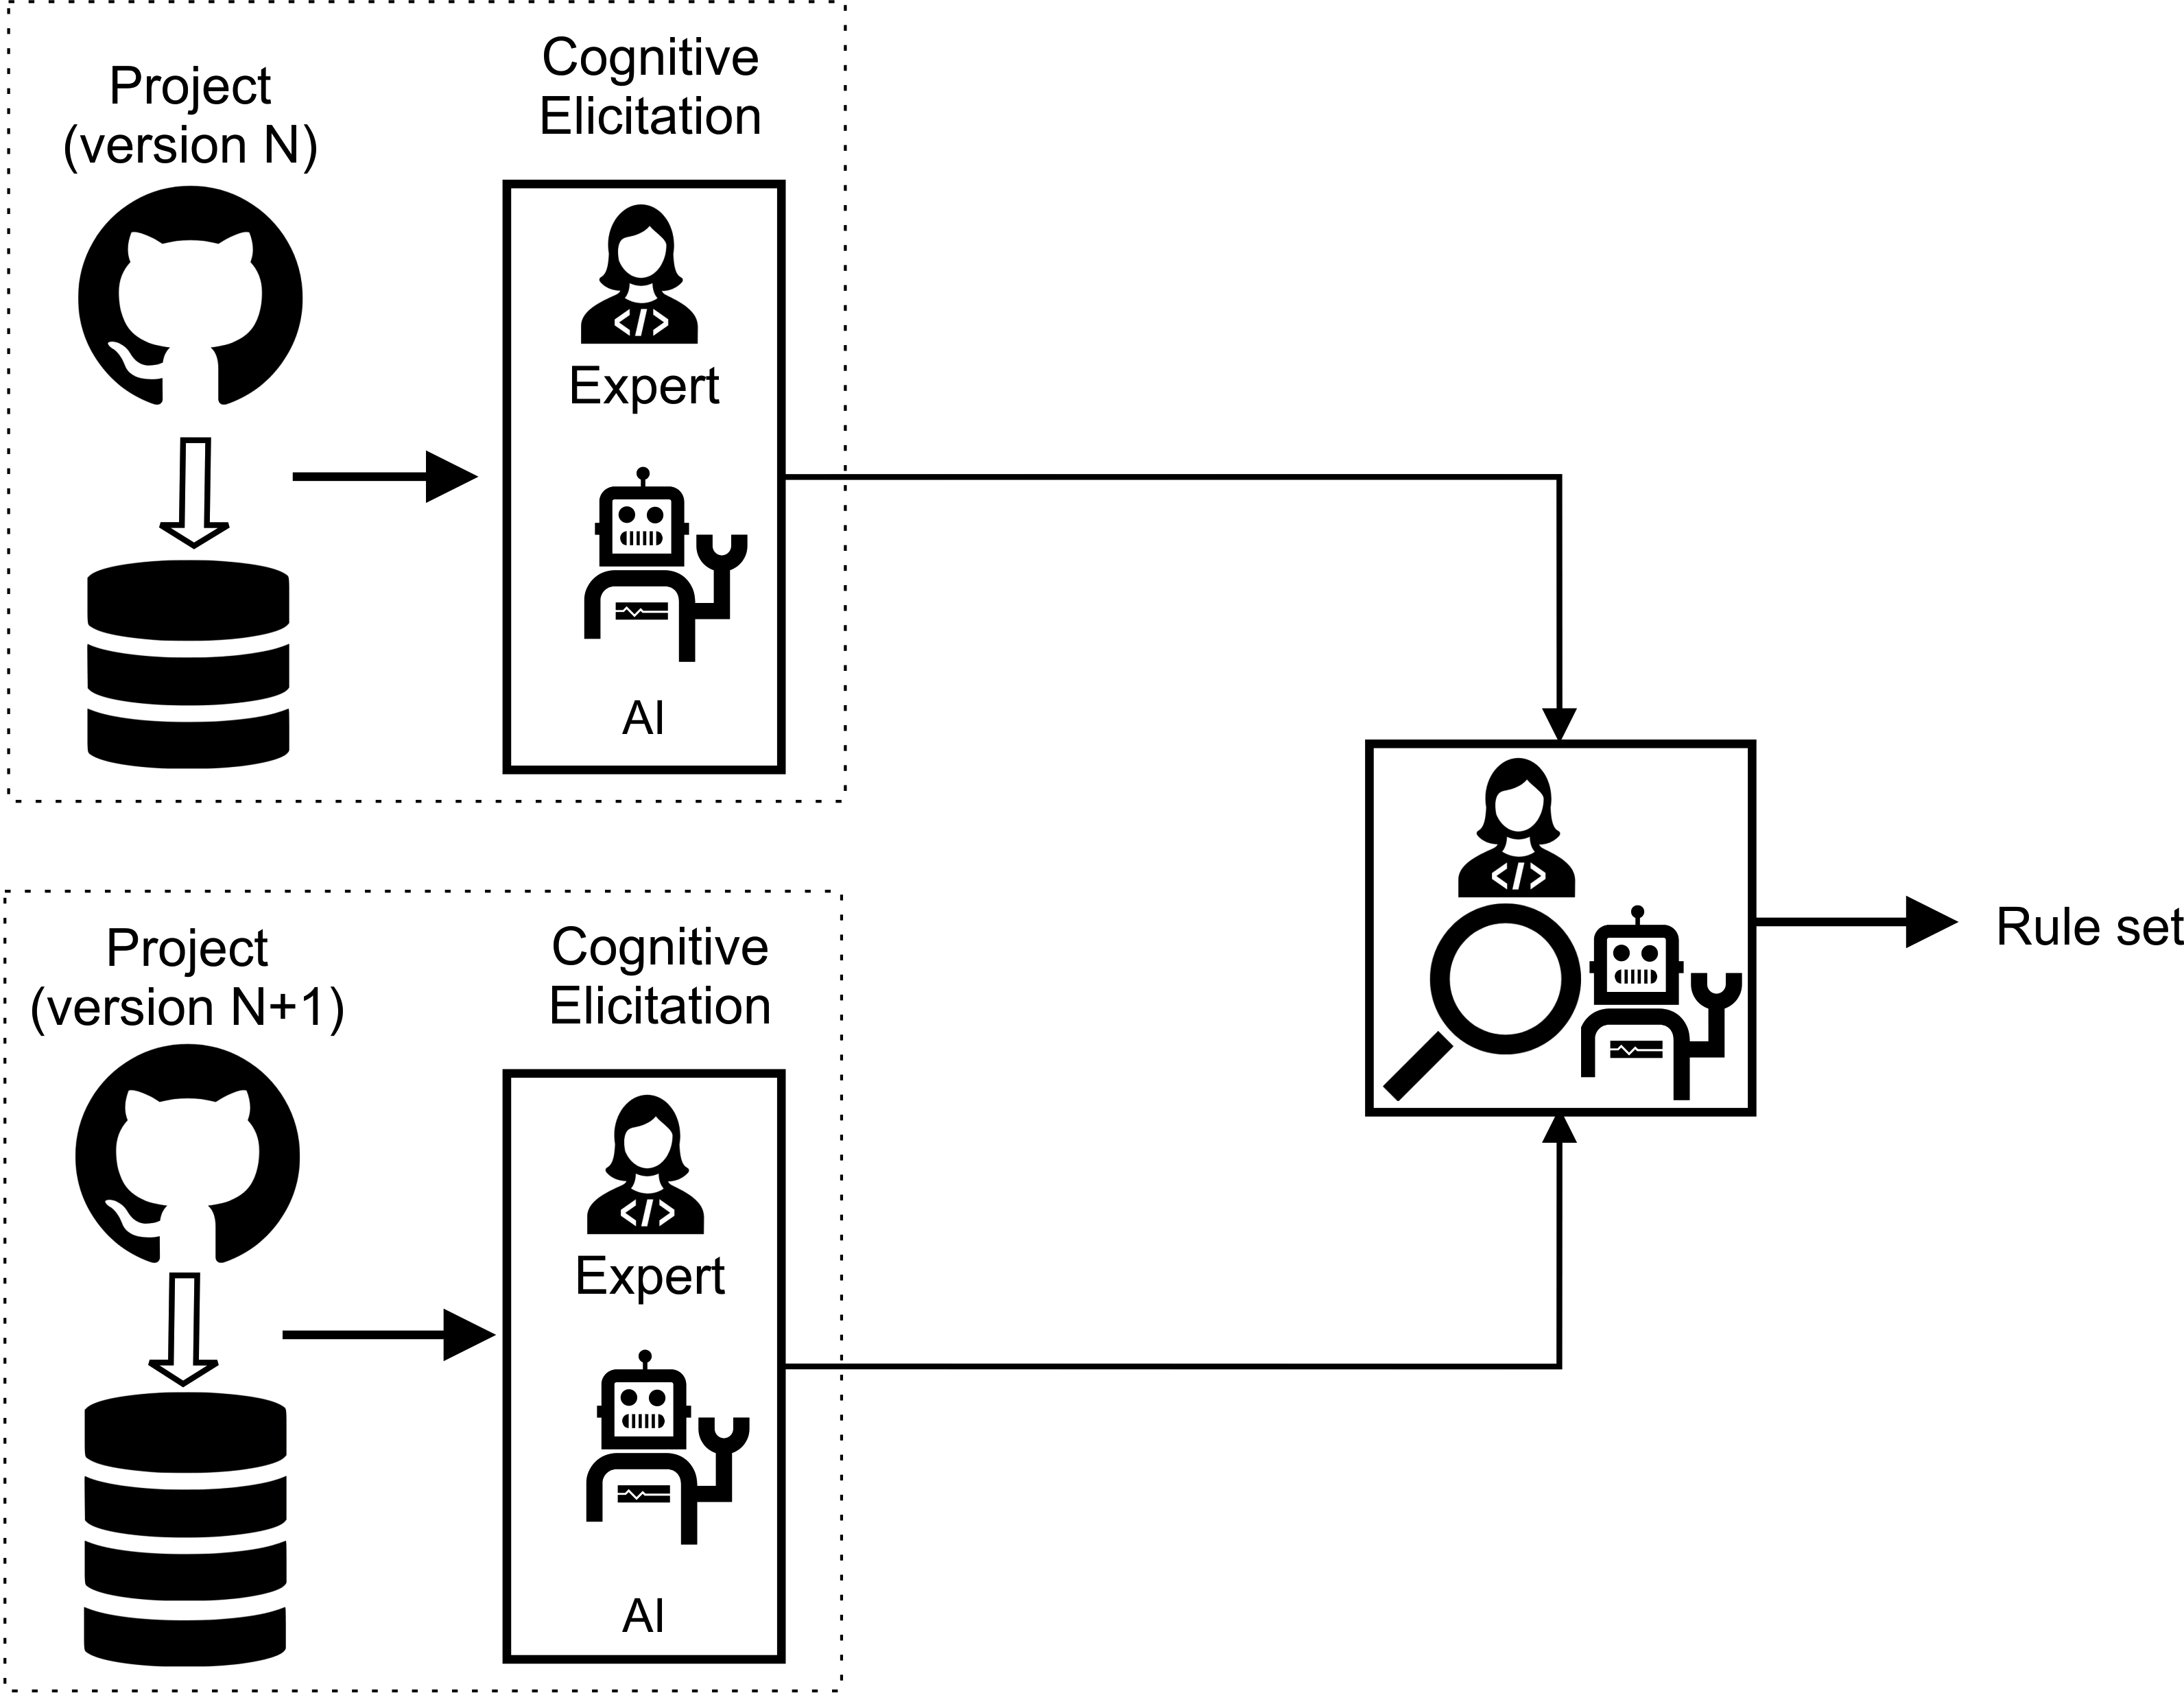
\includegraphics[width=\linewidth]{flow.png}
\caption{Framework for actionable changes.}
\label{fig:xtree}
\end{figure}
\begin{figure}
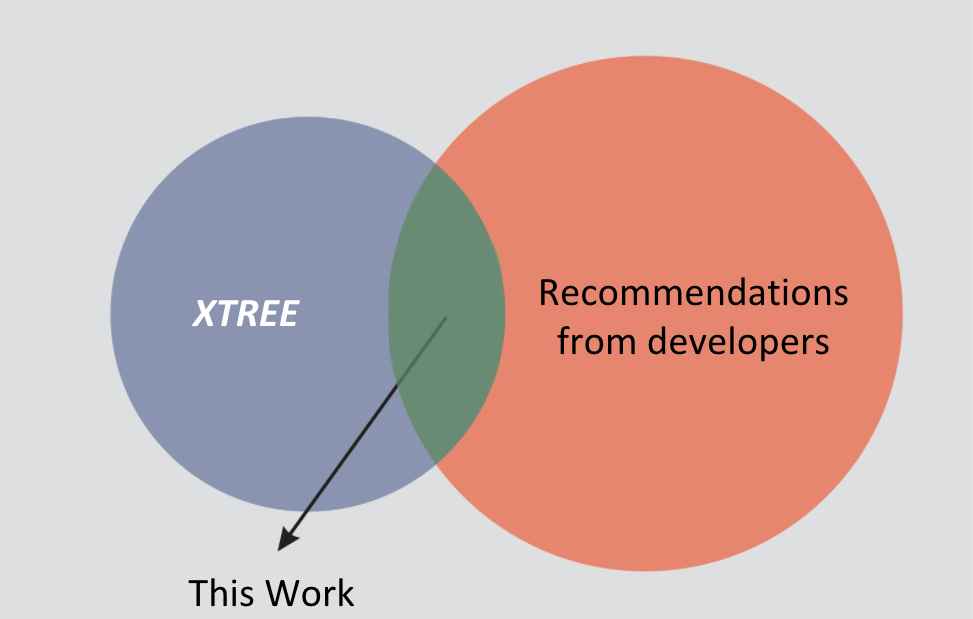
\includegraphics[width=\linewidth]{venn.png}
\caption{Identifying actionable changes.}
\label{fig:xtree}
\end{figure}

\section{Extending XTREE}
\subsection{Why this is necessary?} 
There were some issues with the initial version of XTREE. First, it was limited 
to using data from within a project to generate plans. To address this, we 
developed BELLTREE which used the same framework as XTREE but uses bellwethers 
as the source of data for planning. Our results comparing BELLTREE with XTREE 
on a set of open source java projects as reported in ~\cite{belltree17} was 
that if within-project data from previous releases are 
available, we may use XTREE. If not, using bellwethers would be a reasonable 
alternative. 

However, we noted that XTREE suffered from one major demerit. Which was that it 
recommended plans that were not actionable. For instance, one of the most 
commonly recommended change was to \textit{reduce line of code}. Although, this 
is a plausible action, it is likely that in some cases, developers may not be 
entirely capable of making this change. Therefore, we need to minimized such 
recommendations.

This is very important for reasons discussed in \S2.1. Briefly, generation of 
valid plans precludes other enhancements such as multi-goal reasoning and 
incremental learning. Further, it is also crucial to ensure accurate transfer 
of knowledge.

\subsection{What needs to be done?}
The proposed framework for addressing the issue of actionable conclusion is 
shown in Figure~3. The steps are briefly listed below:
\begin{itemize}
	\item Gather project data and generate plans using an automated approach. In 
	this case, XTREE.
	\item Next, gather expert opinions on what constitutes a doable change.
	\item Finally, combine the rules generated by experts and those generated by 
	XTREE to generate a set of actionable plans.
\end{itemize}  

As shown in Figure~4, we seek the shaded green region. Currently, XTREE 
recommends changes in the \colorbox{steel}{{\color{white}\textbf{blue}}}, 
developers recommendations are shown in 
\colorbox{orange}{{\color{white}\textbf{orange}}}. The subset of desirable 
changes that we seek is shown in \colorbox{Code}{{\color{white}\textbf{green}}}.

\subsection{How this will be achieved?}

This report endorses a four-step procedure to achieve this. These are listed 
below:
\begin{enumerate}
	\item First, we compare the differences between different versions of a 
	project.
	\item Next, we discover the attributes that have most changed between 
	different versions of the project.
	\item After that, we construct an XTREE that are more biased towards the most 
	frequent attributes changed and less so towards the least frequent changes.
	\item Finally, we compare the plans obtained from (3) with plans generated 
	from an unbiased XTREE that allows changes to	everything.
\end{enumerate}

\noindent Figure~5 shows the proposed experimental setup that uses the above 
steps.

\begin{figure}[t!]
\centering
\resizebox{0.9\linewidth}{!}{\begin{tabular}{|p{0.95\linewidth}|}
\hline
Consider a project $\mathds{{X}}$ with versions 
${v}=1,2,3,4,5$. Here:
\begin{enumerate}
	\item First, we use versions $v=1,2$ to identify the most changed 
	features. 
	\item Then we construct the XTREE with version $v=3$ and generate plans for 
	version $v=4$. We call these plans $P_{raw}$. 
	\item Next, we \textit{bias} XTREE with the change frequency information of 
	step (1) and generate different set of plans. We call these plans $P_{bias}$.
	\item Finally, we look at version $v=5$ to compare the plans generated with 
	$P_{raw}$ and $P_{bias}$ and identify the ones most explored by the 
	developers.\vspace{-.4cm}
\end{enumerate}\\\hline
\end{tabular}}
\caption{Proposed experimental procedure.}
\end{figure}

\balance
\bibliographystyle{ACM-Reference-format}
\bibliography{essay}
\end{document}
